\documentclass[10pt,a4paper]{article}
% ready for submission
\usepackage[final]{neurips_2024}

\usepackage[utf8]{inputenc} % allow utf-8 input
\usepackage[T1]{fontenc}    % use 8-bit T1 fonts
\usepackage{hyperref}       % hyperlinks
\usepackage{url}            % simple URL typesetting
\usepackage{booktabs}       % professional-quality tables
\usepackage{amsfonts}       % blackboard math symbols
\usepackage{nicefrac}       % compact symbols for 1/2, etc.
\usepackage{microtype}      % microtypography
\usepackage{xcolor}         % colors
\usepackage[english]{babel}
\usepackage{graphicx}

% decrease page margins
\usepackage{geometry}
\geometry{margin=0.6in}

\title{Variational Autoencoder: A Deep Generative model}
\author{
  Ayush Raina \\
  IISc Bangalore \\
  \texttt{ayushraina@iisc.ac.in} \\
  \And
  Arnav Bhatt \\
  IISc Bangalore \\
  \texttt{arnavbhatt@iisc.ac.in} \\
  \AND
  Anushka Dassi \\
  IISc Bangalore \\
  \texttt{anushkadassi@iisc.ac.in} \\
}

\begin{document}


\maketitle


\begin{abstract}
  Autoencoders are deep generative models. They are widely used for tasks such as image generation, data compression, denoising and capturing the most important features of the data. Autoencoders contains encoder and decoder networks. Variational Autoencoders introduce probabilistic modelling into encoding process in which we learn the latent distribution, which enables generation of data which are similar to training data.
\end{abstract}


\section{Introduction}
A basic knowledge of neural networks is required to understand the further concepts which are convered in this paper.

\subsection{Autoencoder}
This is a neural network which consists of two parts: Encoder($\phi$),Decoder($\theta$) (where $\phi, \theta$ are the parameters)and bottleneck layer whose dimension is much less than input layer. Encoder network learns the latent representation of the input data and decoder network learns to reconstruct the input data from the latent representation. The loss function is defined as the difference between input and output data.

\subsection{Aim}
We want output of the network as input itself. The main challenge is that input has to pass from a bottleneck layer whose dimension is much less than input layer. We can say that the network learns to compress the data to hidden state.

\subsection{Objective Function}
In this case we are dealing with images and we want our output image to be as similar as input image. Since our image passes through encoder and decoder network we can set up the loss function as follows:

% \begin{equation} in box
\[
  min \;\; \sum_{i=1}^{m} ||\;  x^{(i)} - Decoder_{\theta}(Encoder_{\phi}(x^{(i)})) \; ||^2
\]

\section{Expectation Maximization (EM) Algorithm}
EM algorithm is used to perform the maximum likelihood estimation in the presence of latent variables. This is a two step process consisting of E-step and M-step. Suppose $\psi$ are the parameters we want to learn and $z^{(i)}$ are the latent variables. Then we perform these two steps iteratively until convergence: \\
E-step: For all $i$, set $Q_i(z^{(i)}) = p(z^{(i)}|x^{(i)}; \psi)$, M-step: $\psi^{(new)}$ = $argmax_{\psi} \sum_{i=1}^{m} ELBO(x^{(i)};Q_i,\psi)$, where ELBO is called evidence lower bound. The problem in this algorithm is that in E-step, we assumed that the posterior distribution $p(z^{(i)}|x^{(i)}; \psi)$  can be calculated, but sometimes it may be extremely complex to calculate this distribution, for example suppose $z \sim N(0,I_{k \times k})$ and $x | z \sim NeuralNetwork(z^{(i)};\theta)$, then it is almost impossible to calculate the posterior distribution $p(z^{(i)}|x^{(i)}; \psi)$ because of the complexity of the neural network.
\\ So we need to find a way to approximate this distribution. There are many ways to approximate this distribution, like Gibbs sampling, Variational Inference, etc. In this paper we will discuss about the variational inference.

\section{Variational Inference}
We know that $log(P(x)) = ELBO(x;Q) + D_{KL}(Q || P_{z|x})$, where $ELBO(x;Q) = E_{z \sim Q} [log(\frac{log(P(x,z)}{Q(x)}]$ and $D_{KL}(Q || P_{z|x})$ is the KL Divergence between the $Q$ and the true posterior distribution $P_{z|x}$. We want $Q$ to be as close as possible to the true posterior distribution $P_{z|x}$, which mean $D_{KL}(Q || P_{z|x}) \longrightarrow 0$. So if we maximise the ELBO with respect to $Q$, then we are minimising the KL Divergence between $Q$ and $P_{z|x}$, because the $log(P(x))$ is constant. So we can say that $P_{z|x} \sim argmax_{q \sim Q} ELBO(x;q)$, where we will assume all $q's$ are in the same family of distributions($Q$) called as variational family. These are distributions over vectors of dimension $k$. In our case we will also assume that $Q$ is a family of Gaussian distributions.

\subsection{Mean Field Variational Inference}
Sometime for the ease of computation we assume that variational family $Q$ factorizes, so that $Q(z) = \prod_{i=1}^{k} q_i(z^{(i)})$, which means each latent variable $z^{(i)}$ is independent. This assumption is called mean field assumption and the method is called mean field variational inference. 

\section{Autoencoders again}
\subsection{Generation with Autoencoders}
Till now we have seen that autoencoders take input and maps it to hidden representation(latent representation) and decoder reconstructs the input back from the hidden representation. After the training, we can remove the encoder part and feed random latent representation to the decoder to generate output. But we may not get meaningful outputs because latent representations lies in very small subspace of the input space.\\
To generate meaningful outputs we need to feed the latent variables which is similar to the training data. In other words we want latent variables to be sampled from $P(z|X)$.But autoencoders learn hidden representation $z$ but not a distribution $P(z|X)$. Same is in the case of decoder every time we feed the same latent representation we get the same output, which means both encoder and decoder are deterministic in this case. Now we will look over \textcolor{red}{Variational Autoencoders} which have same structure but they learn the distribution over the latent variables.

\section{Variational Autoencoders}
We are interested in $P(z|X)$ which corresponds to learning hidden representation. Variational Autoencoders use encoders to learn this distribution by method of variational inference. We will assume that our variational family $Q$ is Gaussian and encoder network will give us the mean and variance of this distribution. Hence $Q = N(\mu(X), \Sigma(X))$ where $\mu(X), \Sigma(X) = Encoder_{\phi}(X)$. Note that $\mu(X), \Sigma(X)$ are functions of input $X$. Once we learned this distribution we can sample from this distribution and feed this sample to the decoder to generate the output. Here is the visual representation of the model:

\begin{figure}[h]
    \centering
    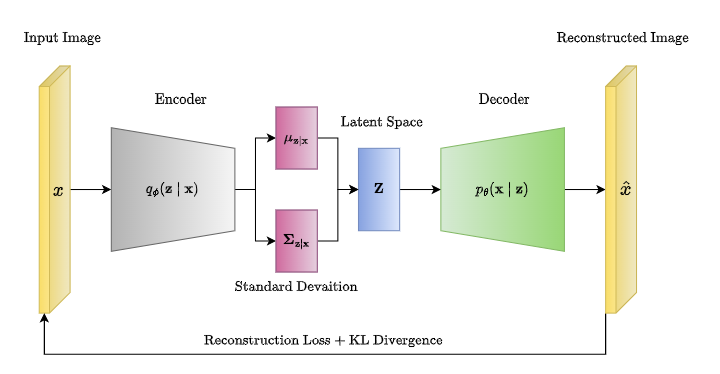
\includegraphics[width=0.5\textwidth]{vae.png}
    \caption{Variational Autoencoder}
    \label{fig:my_label}
\end{figure}

\section{Experimental Results and Conclusions}

\end{document}